% 例 2：菱形 ABCD, ∠BAD = 60°, AB = 4
% 取 A 在左、对角线 BD 竖直、AC 水平的对称摆法
% ∠BAD = 60°, 对角线 AC 平分 ∠BAD → ∠BAO = 30°
% 在 Rt△AOB 中 ∠BAO=30°, AB=4 → OB=2, OA=2√3
\documentclass[tikz,border=4pt]{standalone}
\usepackage{ctex}
\usepackage{amsmath}
\usetikzlibrary{calc, angles, quotes, decorations.markings}
\begin{document}
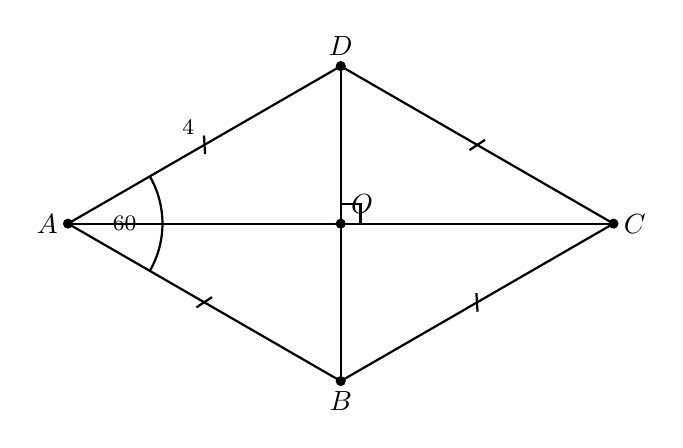
\begin{tikzpicture}[scale=1.0, thick,
  tickone/.style={postaction={decorate, decoration={markings,
    mark=at position 0.5 with {\draw (-1.5pt,-3pt) -- (1.5pt,3pt);}}}},
]
  \def\OA{3.464} % 2*sqrt(3) ≈ 3.464
  \coordinate (A) at (-\OA,0);
  \coordinate (B) at (0,-2);
  \coordinate (C) at (\OA,0);
  \coordinate (D) at (0,2);
  \coordinate (O) at (0,0);
  \draw[tickone] (A) -- (B);
  \draw[tickone] (B) -- (C);
  \draw[tickone] (C) -- (D);
  \draw[tickone] (D) -- (A);
  \draw (A) -- (C);
  \draw (B) -- (D);
  \draw (0.25,0) -- (0.25,0.25) -- (0,0.25);
  \draw pic[draw, angle radius=12mm, "$60°$" font=\footnotesize] {angle = B--A--D};
  \foreach \pt in {A,B,C,D,O} \filldraw (\pt) circle (1.4pt);
  \node[left]  at (A) {$A$};
  \node[below] at (B) {$B$};
  \node[right] at (C) {$C$};
  \node[above] at (D) {$D$};
  \node[above right] at (O) {$O$};
  \node[font=\footnotesize, above left] at ($(A)!0.5!(D)$) {$4$};
\end{tikzpicture}
\end{document}
